\chapter*{Presentasi Makalah}

\begin{figure}[h]
  \centering
  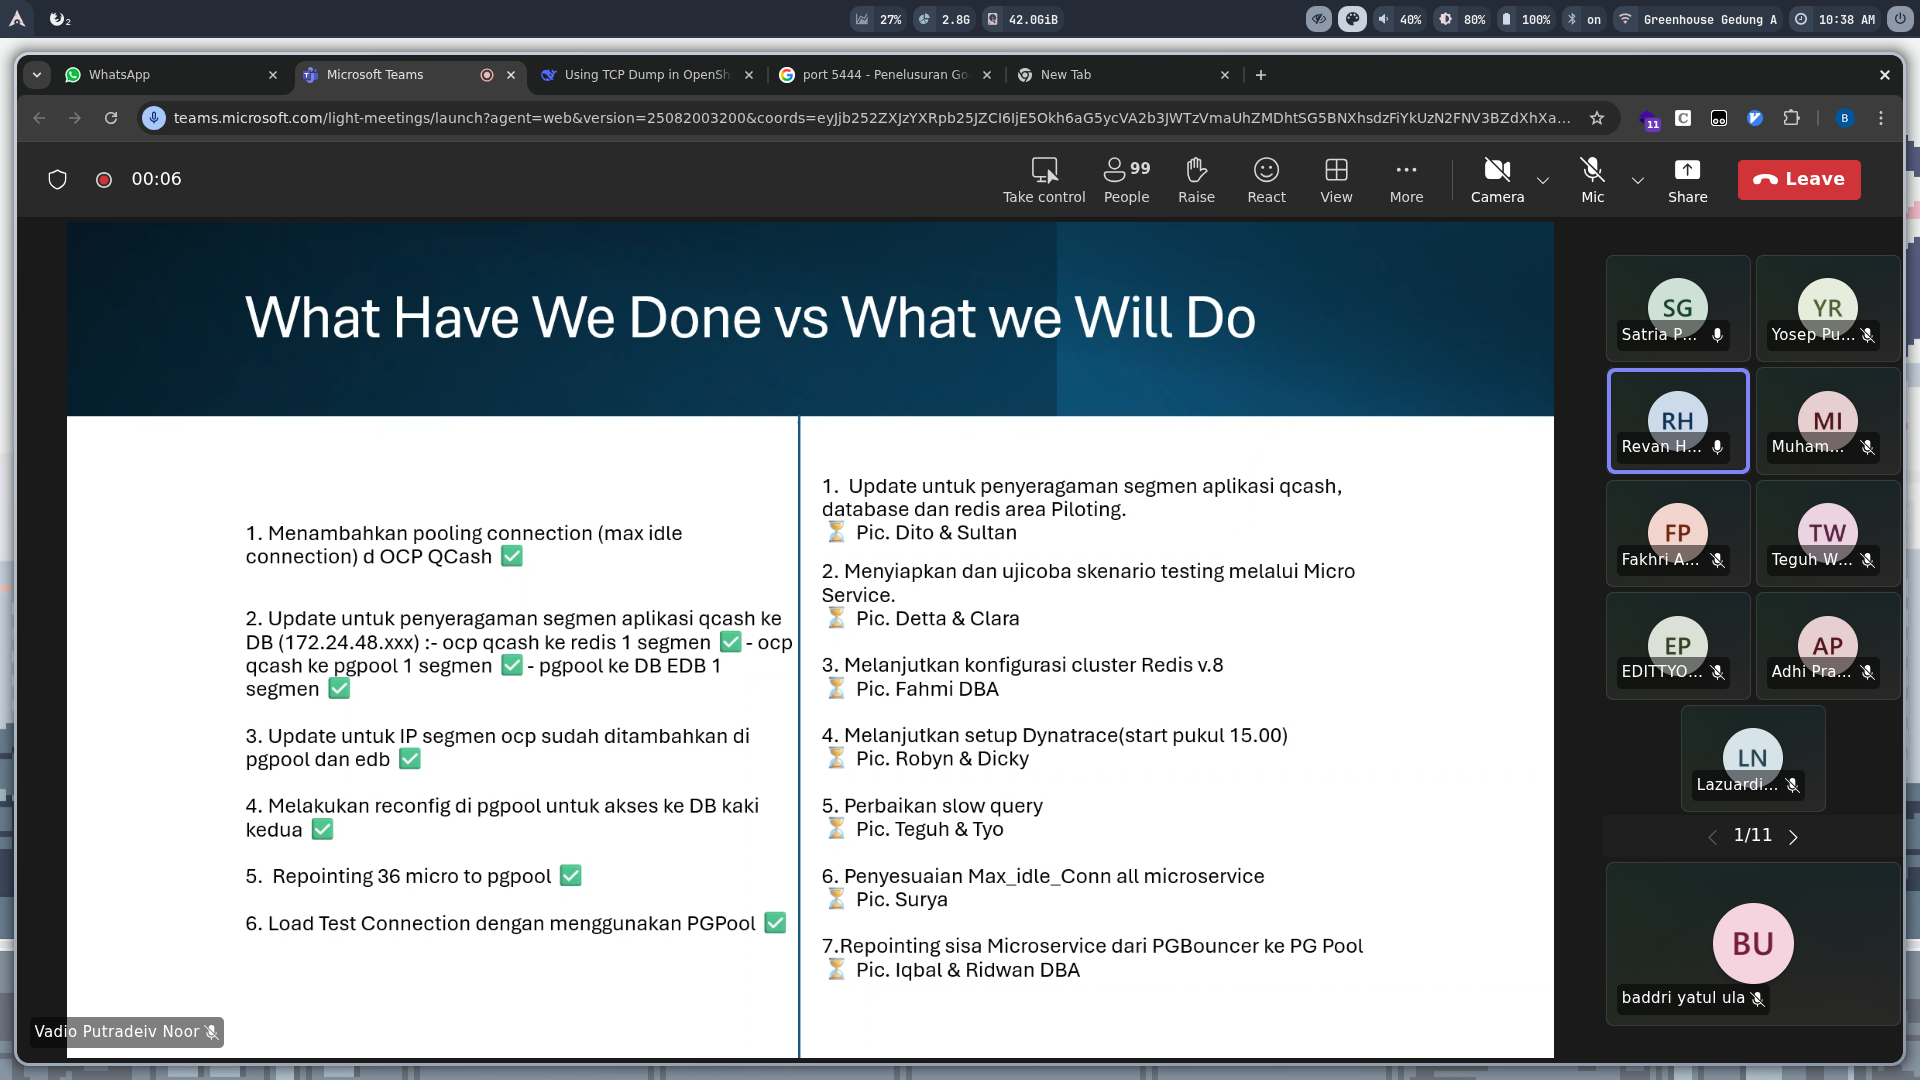
\includegraphics[width=1\textwidth]{images/fig1.png}

  \raggedright
  {\footnotesize \textit{Source: Author’s illustration}}%
  \par
  %   \vspace{2pt}

  \caption{Insiden QCash November 2025}
  \label{fig:fig1}
\end{figure}

\begin{table}[h]
  \centering
  \caption{Example of a four-column table}
  \label{tab:example}
  \begin{tabular}{ l c r p{4cm} }
    \toprule
    \textbf{Left} & \textbf{Center} & \textbf{Right} & \textbf{Paragraph Column} \\
    \midrule
    Apple  & 10   & 100   & This is a longer description that wraps to multiple lines. \\
    Banana & 20   & 200   & Another text entry with wrapping. \\
    Cherry & 30   & 300   & Short note. \\
    \bottomrule
  \end{tabular}
  \vspace{4pt}
\end{table}

\begin{table}[h]
  \centering
  \caption{CPU allocation by pod}
  \label{tab:cpu}
  \begin{tabular}{l c l c}
    \toprule
    \textbf{Pod} & \textbf{CPU Request (m)} & \textbf{Status} & \textbf{Is Available} \\
    \midrule
    frontend & 500 & Good & Yes \\
    backend  & 250 & Fine & No \\
    database & 1000 & Better & Yes \\
    \bottomrule
  \end{tabular}

  \vspace{4pt}
  {\footnotesize \textit{Note:} $m$ stands for millicore, where $1000m = 1$ CPU core.}
\end{table}
